%----------------------------------------------------------------------------------------
%    INSTRUMENTS ÒPTICS
%----------------------------------------------------------------------------------------
\section{Instruments òptics}
\subsection{Ull humà}
\begin{figure}[H]
\centering
    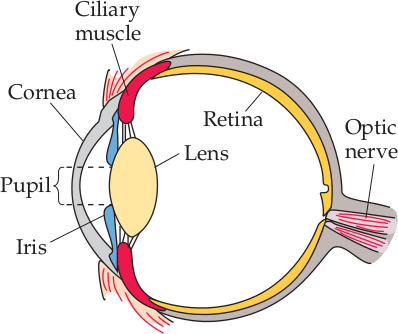
\includegraphics[width=0.5\textwidth]{images/5/51-ull.png}
\caption{Diagrama de l'ull humà}
\end{figure}

\subsubsection*{Característiques òptiques de l'ull}
\begin{itemize}
    \item Pupil·la: Té un diàmetre variable de $\sim \SIrange[range-phrase= -]{2}{8}{\mm}$.
    \item Cristal·lí: $n_{C} \approx \numrange[range-phrase = -]{1.386}{1.406}$ (enfoc variable).
        \subitem Cons: cèl·lules fotosensibles que permeten distingir els colors. N'hi ha $\sim \numrange[range-phrase = -]{6e6}{7e6}$.
        \subitem Bastons: cèl·lules fotosensibles que capten l'intensitat de llum. N'hi ha $\sim 125 \times 10^{6}$.
    \item Còrnia: quan el cristal·lí està relaxat, la distància focal del sistema còrnia--cristal·lí és de $\SI{2.5}{cm}$, que és la distància entre la còrnia i la retina.
    \item Humor aquós i vitri: $n_{A} \approx 1.336$, $n_{V}\approx 1.336$.
    \item Punt proper ($x_{pp}$): és el punt més proper pel qual el cristal·lí pot enfocar la imatge a la retina. S'agafa $\SI{25}{\cm}$ com a valor estàndard.
\end{itemize}

\subsubsection*{Defectes de l'ull}
\begin{itemize}
    \item Miopia: la imatge es forma abans de la retina. S'arregla amb lents divergents.
    \item Hipermetropia: la imatge es forma després de la retina. S'arregla amb lents convergents.
    \item Presbícia: la distància més propera disminueix.
\end{itemize}

\subsubsection*{Mida aparent d'un objecte}
\begin{figure}[H]
\centering
    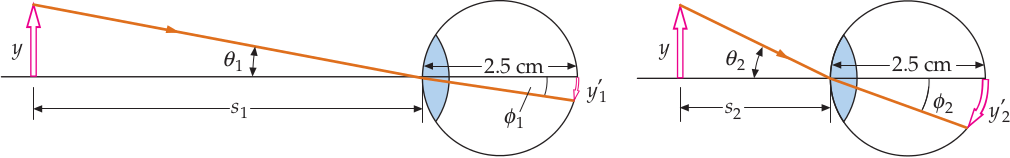
\includegraphics[width=\textwidth]{images/5/51-ull-imatge.png}
\caption{Diagrama de formació d'imatges sobre la retina de l'ull. Un objecte llunyà sembla petit perquè la seva imatge és més petita que la del mateix objecte més proper a l'ull}
\end{figure}
\begin{align}
    \boxed{\phi = \frac{y'}{\SI{2.5}{\cm}}} \quad \boxed{\theta \approx \frac{y}{s}}
\end{align}
Aplicant la llei d'Snell per a la refracció, tenim que $n_{aire} \sin \theta = n \sin \phi$, on $n$ és l'índex de refracció de l'interior de l'ull. Llavors, per a angles petits:
\begin{align}
    \boxed{\theta \approx n \phi}
\end{align}
Així doncs, combinant les equacions anteriors, tenim:
\begin{align}
    \boxed{y' = \frac{\SI{2.5}{\cm}}{n} \frac{y}{s}}, \quad s \geq x_{pp} = \SI{25}{\cm}
\end{align}

%----------------------------------------------------------------------------------------
\subsection{Magnificador simple}
Una lent convergent s'anomena magnificador simple o lupa si se situa a prop de l'ull i si l'objecte se situa de la lent a una distància inferior a la seva distància focal.
\begin{figure}[H]
\centering
    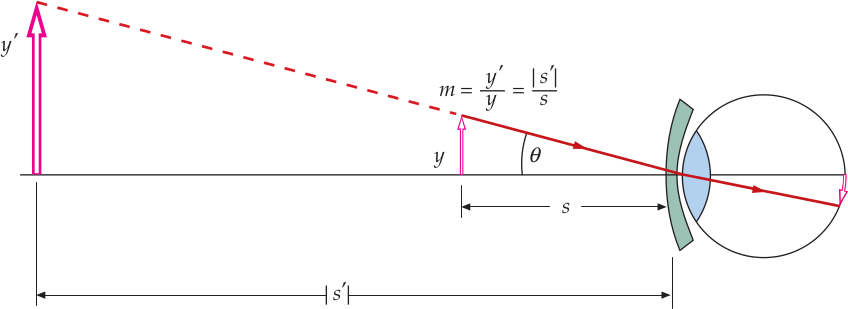
\includegraphics[width=\textwidth]{images/5/52-magnificador.png}
\caption{Diagrama de rajos d'un magnificador simple}
\end{figure}
Per a l'ull, la imatge d'un objecte subtendeix un angle $\theta$ donat per aproximadament:
\begin{align}
    \boxed{\theta \approx \frac{y}{s} = \frac{y'}{|s'|}}
\end{align}
\subsubsection*{Poder magnificador}
L'angle màxim que pot subtendir l'ull és $\begin{gathered}\theta_{o} = \frac{y}{x_{pp}}\end{gathered}$ (amb l'objecte al punt proper), però quan posem al davant un magnificador simple, aquest angle màxim augmenta fins a $\begin{gathered}\theta = \frac{y}{f}\end{gathered}$ (posant l'objecte a la distància focal). 

Llavors, definim el poder magnificador o amplificació angular d'una lent com a:
\begin{align}
    \boxed{M = \frac{\theta}{\theta_{o}} = \frac{x_{pp}}{f}}
\end{align}
Aleshores, un magnificador simple permet enfocar objectes a una distància molt propera (de manera que la seva imatge formada a la retina és major) amb l'ull relaxat.

%----------------------------------------------------------------------------------------
\subsection{Microscopi compost}
\begin{figure}[H]
\centering
    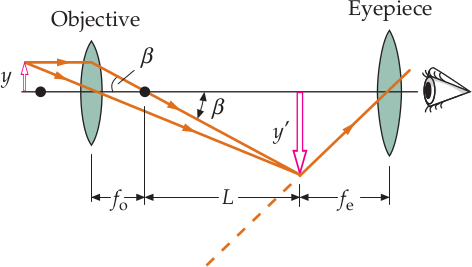
\includegraphics[width=0.6\textwidth]{images/5/53-microscopi.png}
\caption{Diagrama de rajos d'un microscopi òptic compost. Està composat per, d'esquerra a dreta un objectiu i un ocular}
\end{figure}
La magnificació lateral $m_{o}$ de l'objectiu és:
\begin{align}
    \boxed{m_{o} = \frac{y'}{y} = - \frac{L}{f_{o}}}
\end{align}
on $f_{o}$ és la distància focal de l'objectiu i $L$ és la distància entre la focal de l'objectiu i la focal de l'ocular; l'anomenem distància del tub.

El poder magnificador de l'ocular és:
\begin{align}
    \boxed{M_{e} = \frac{x_{pp}}{f_{e}}}
\end{align}
El poder magnificador del sistema compost és el producte dels augments de l'objectiu i l'ocular:
\begin{align}
    \boxed{M = m_{o} M_{e} = - \frac{L}{f_{o}} \frac{x_{pp}}{f_{e}}}
\end{align}

\subsubsection*{Valors estàndard dels augments}
\begin{itemize}
    \item $m_{o}$: $4 \times$, $10 \times$, $20 \times$, $40 \times$, $100 \times$.
    \item $M_{e}$: $10 \times$, $20 \times$.
\end{itemize}

%----------------------------------------------------------------------------------------
\subsection{Telescopi}
\begin{figure}[H]
\centering
    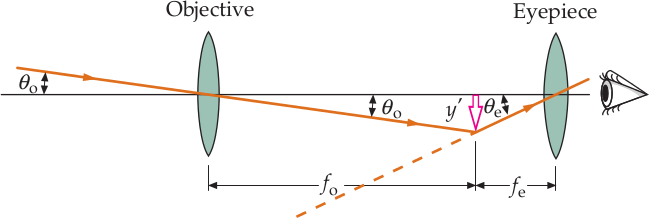
\includegraphics[width=0.8\textwidth]{images/5/54-telescopi.png}
\caption{Diagrama de rajos d'un telescopi}
\end{figure}
Podem fer les aproximacions per a angles petits següents:
\begin{align}
    \boxed{\tan \theta_{o} = \frac{y}{s} = - \frac{y'}{f_{o}} \approx \theta_{o}}
\end{align}
\begin{align}
    \boxed{\tan \theta_{e} = \frac{y'}{f_{e}} \approx \theta_{e}}
\end{align}
com que $y'$ és negativa, $\theta_{e}$ és negativa, indicant que la imatge és invertida.

El poder de magnificació del telescopi és, llavors:
\begin{align}
    \boxed{M = \frac{\theta_{e}}{\theta_{o}} = \frac{f_{o}}{f_{e}}}
\end{align}

\subsubsection*{Telescopi reflector}
\begin{figure}[H]
\centering
    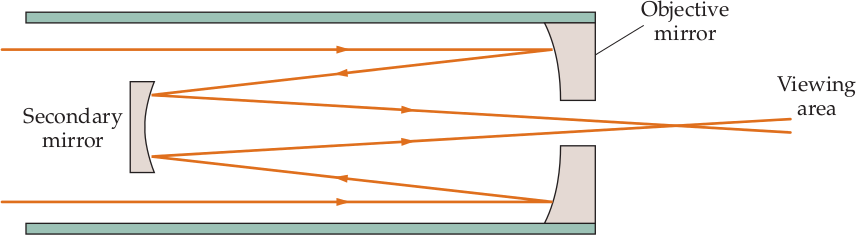
\includegraphics[width=0.9\textwidth]{images/5/54-telescopi-reflector.png}
\caption{Diagrama de rajos d'un telescopi reflector }
\end{figure}
Un telescopi reflector utilitza miralls còncaus en comptes de lents per a l'objectiu. El fet d'utilitzar un mirall té molts avantatges, com ara eliminar la aberració cromàtica.

\subsubsection*{Telescopi de Galileu}
WIP: stuff.